 \documentclass[twocolumn,a4,UTF8]{ctexart} 
\usepackage{amsmath, amsthm}
\usepackage{indentfirst}
\usepackage{listings,xcolor}
\usepackage{geometry} % 设置页边距
\usepackage{fontspec}
\usepackage{graphicx}
\usepackage{float} %设置图片浮动位置的宏包
\usepackage{subfigure} %插入多图时用子图显示的宏包
\usepackage{fancyhdr} % 自定义页眉页脚
%\setsansfont{Consolas} % 设置英文字体
 \pagestyle{fancy}
\setlength{\parindent}{2em}
 \title{创新实践进度报告}
 \author{罗汉东,李龙}
 \date{\today}
  \fancyhf{}
  \lhead{创新实践进度报告}
  \rhead[\nouppercase{\rightmark}]{\thepage}
  \begin{document}
  \maketitle
  \tableofcontents
  \section{最初设计}
 最初的想法是将跑在服务器上实现对图像和文字的识别和处理的神经网络,移植树莓派,利用树莓派的排线摄像头和外接对应针脚的麦克风,之后因为树莓派机能的原因,神经网络在树莓派上的响应性和稳定性均不是太理想
 \section{改进设计}
 	之后打算采用分布式系统的方案,将树莓派只用于采集图像,将手机作为中转站,转发来自树莓派的图像数据到云端,开发了一个简单的安卓app用于从树莓派中获取图像图像
 	\begin{figure}[H] 
	\centering 
	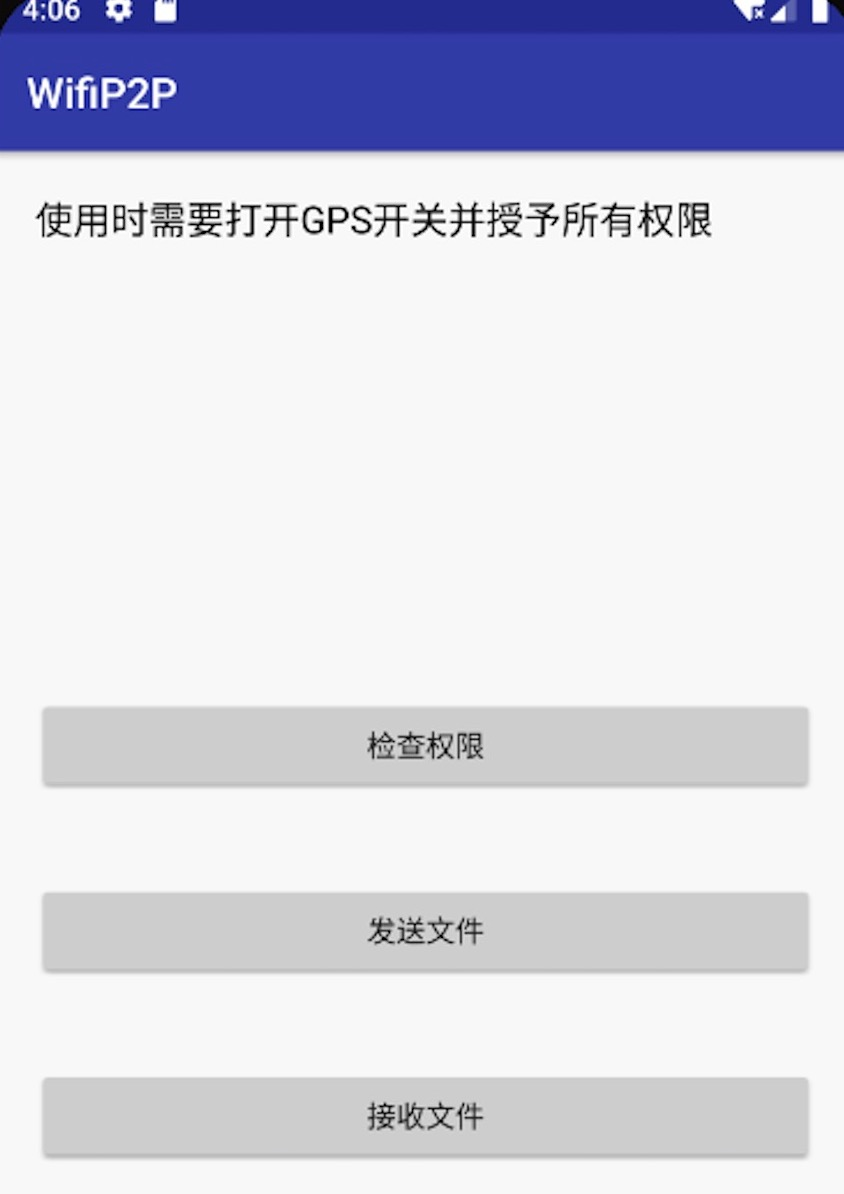
\includegraphics[width=0.4\textwidth]{app.png} 
	\end{figure}
 	\subsection{关于传输瓶颈的改进}
 	之前打算使用蓝牙进行传输,但是由于蓝牙协议的速率不能很好的满足图片文件的即时传输(树莓派上的蓝牙2.3只支持23kb/s的文件传输),之后打算采用类似于AirDrop的传输方案,即先用蓝牙进行握手和交换秘钥,之后使用WIFI-Direct进行图像传输。
 	\begin{figure}[H] 
	\centering 
	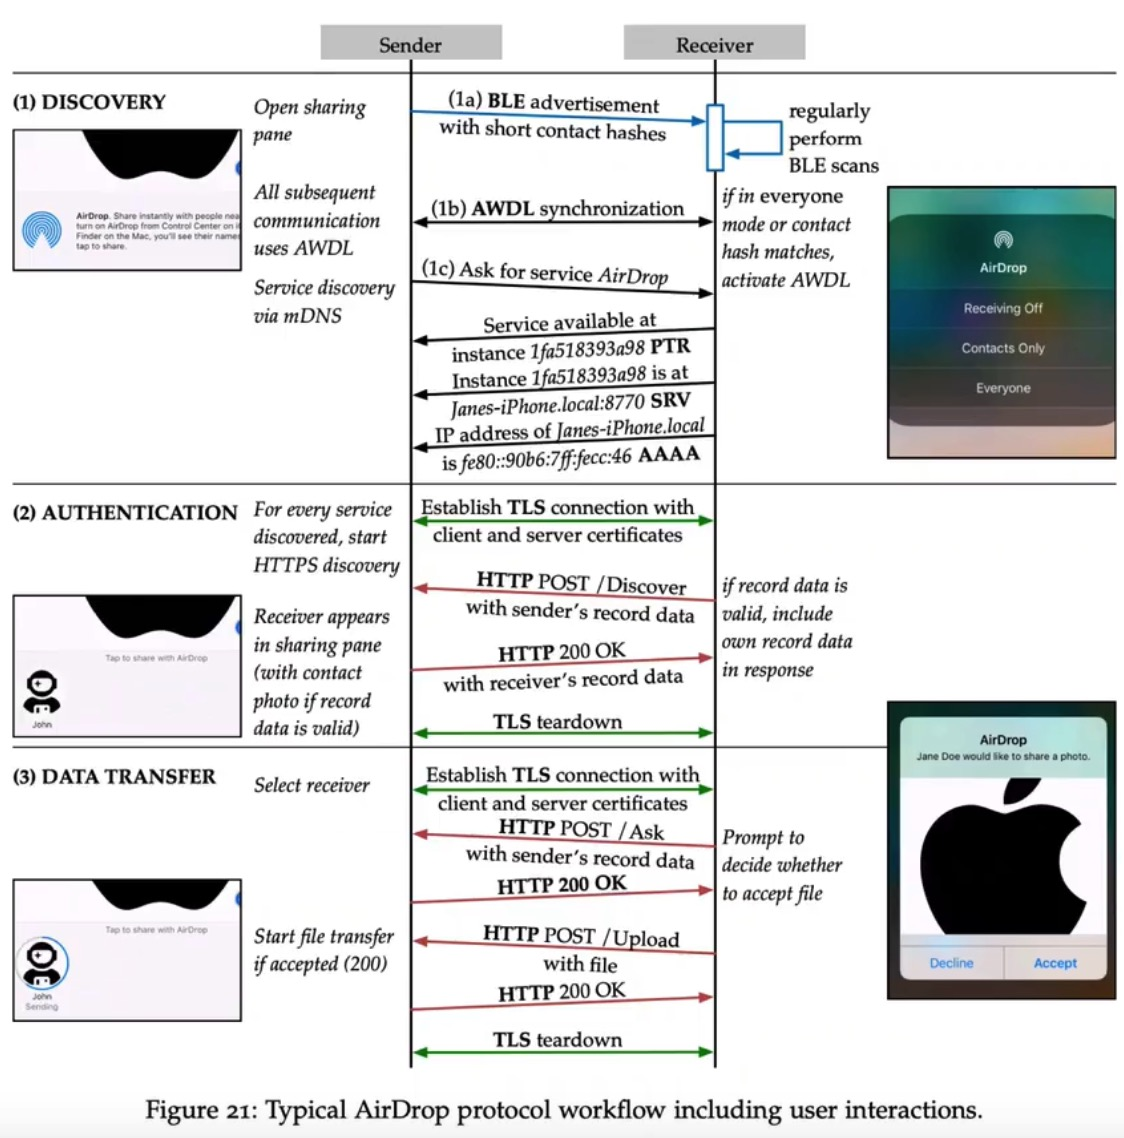
\includegraphics[width=0.4\textwidth]{AirDrop.png} 
	\end{figure}
	\subsection{对于模型进行简化}
	由于WIFI-Driect协议较新,市面上的方案都是各家手机厂商的定制方案,对于开发App来讲,实现WIFI-Direct需要对每家厂商都进行适配,而且现在并没有一个通用的标准以及系统接口来实现对应的功能。
	
	
	改进之后的方案将手机的在整个链路的作用简化成一个网络节点,由树莓派直接对服务器发出请求和接受相应的数据,具体实现就是利用手机的网络AP功能或者USB网络共享功能将树莓派接入手机网络中。
	\begin{figure}[H] 
	\centering 
	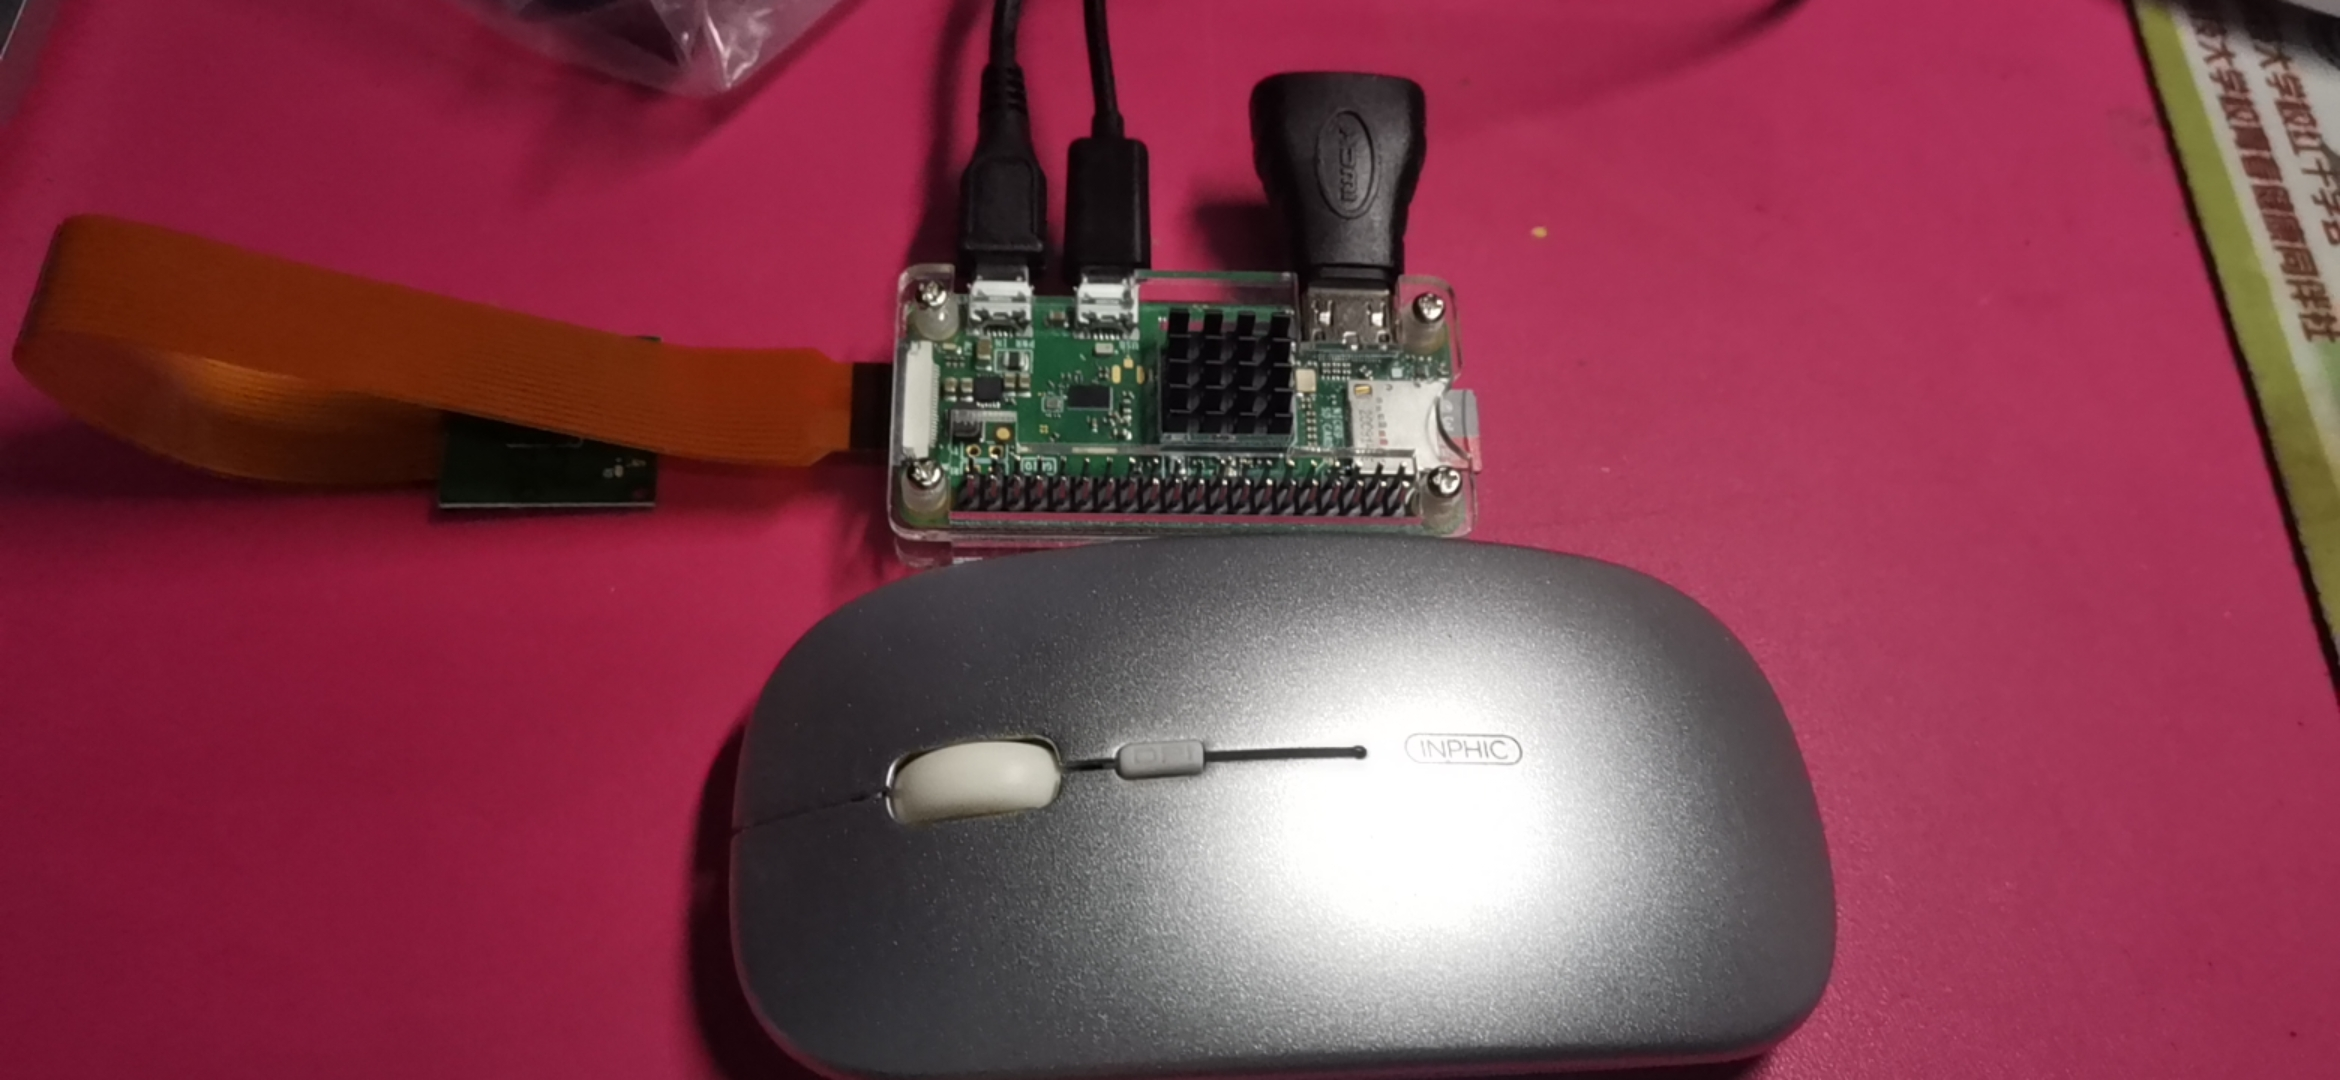
\includegraphics[width=0.4\textwidth]{size.jpg} 
	\end{figure}
	并且现在可以利用小型化的Raspberry pi zero来将整个设备缩小到可穿戴的尺寸。
	\subsection{未实行的改进}
		由于阿里云的服务器端经常宕机,截至9月26号依然无法访问,而且只能提供简单的文字中转的服务,数据传输时需要将图片上传到图床,这会对隐私和整个系统的稳定性造成影响,如果采用ipv6协议,将主服务器的ip解析至域名的AAAA记录,即可实现直连。
		不足之处在于现在ipv6虽然已经普及,但是不能否认还有可能的兼容性问题出现。
	\section{工作进度}
		目前能够使用Python脚本对服务器进行交互,对图床上已有的图片进行操作,但是由于服务器宕机无法进行进一步调试验证,即实现从本地上传图片到图床,再发送指令到服务器进行操作。
		\subsection{对可穿戴设备外壳的设计}
		目前的外壳采用3D打印方案,类似于Google glass的的设计,将树莓派和其摄像头安置于眼睛中框和侧边。
		\begin{figure}[H] 
	\centering 
	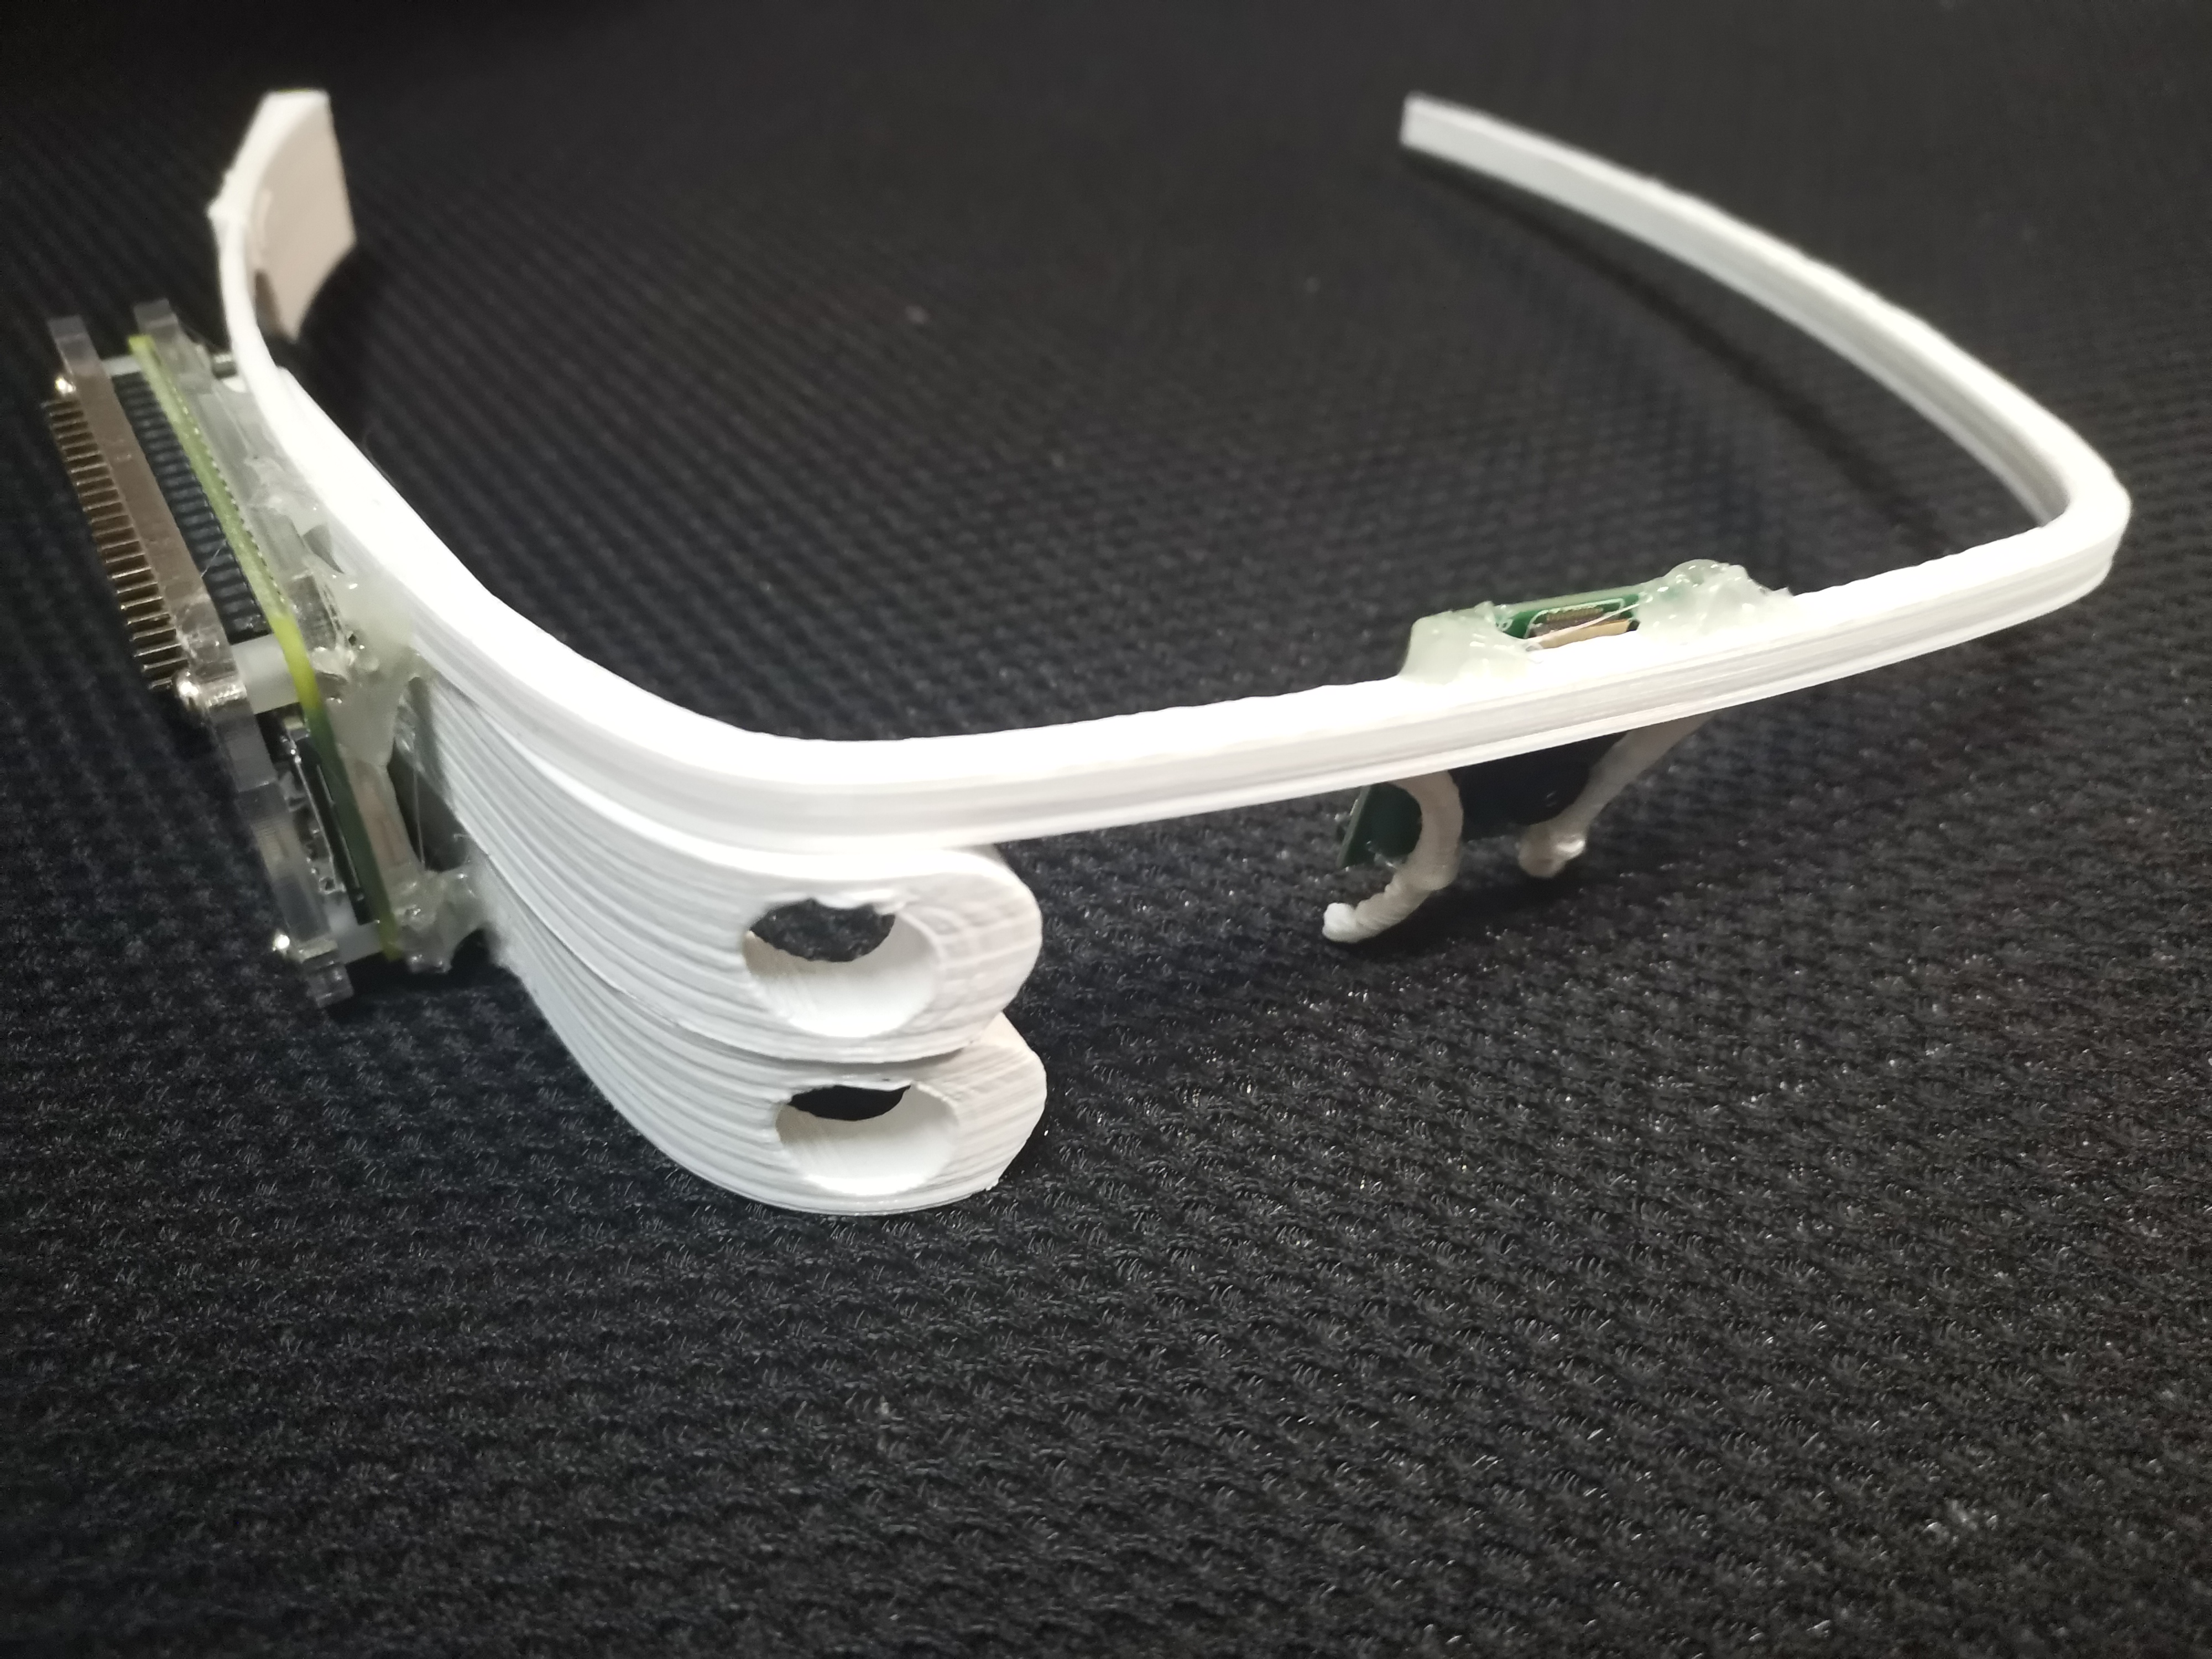
\includegraphics[width=0.4\textwidth]{glassfront.jpg} 
	\end{figure}
		但是由于还需要考虑电池以及其保护外壳大小的原因,不排除重新设计的可能,一种可能是将中框的一部分改造成电池,但是这样对部件的强度要求较大.
	\subsection{树莓派外接交互按钮、声音输出接口的设计以及驱动编写}
		由于树莓派自带的Broadcom BCM2835芯片并不含DA转换功能。
		\begin{figure}[H] 
	\centering 
	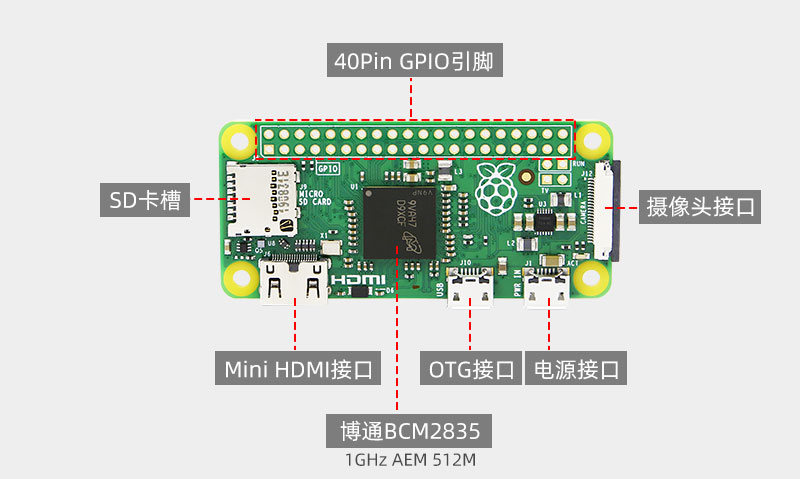
\includegraphics[width=0.4\textwidth]{zero.png} 
	\end{figure}
		目前可行的方案可以通过其PWM引脚实现软件模拟输出,但是PWM引脚的工作频率是在50khz,需要低通滤波才能使用,而且缺乏静电保护等必要电路,需要将这一部分电路外挂,目前尚未制板。
			\begin{figure}[H] 
	\centering 
	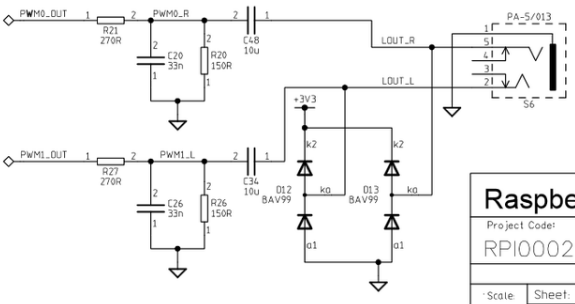
\includegraphics[width=0.4\textwidth]{dianlu.png} 
	\end{figure}
	\subsection{供电电路以及电池的设计}
	对于树莓派的供电可以使用其自带的microUSB接口进行供电,但是这会影响树莓派的USB扩展性,以及USB线会占用可穿戴设备宝贵的体积。
	\begin{figure}[H] 
	\centering 
	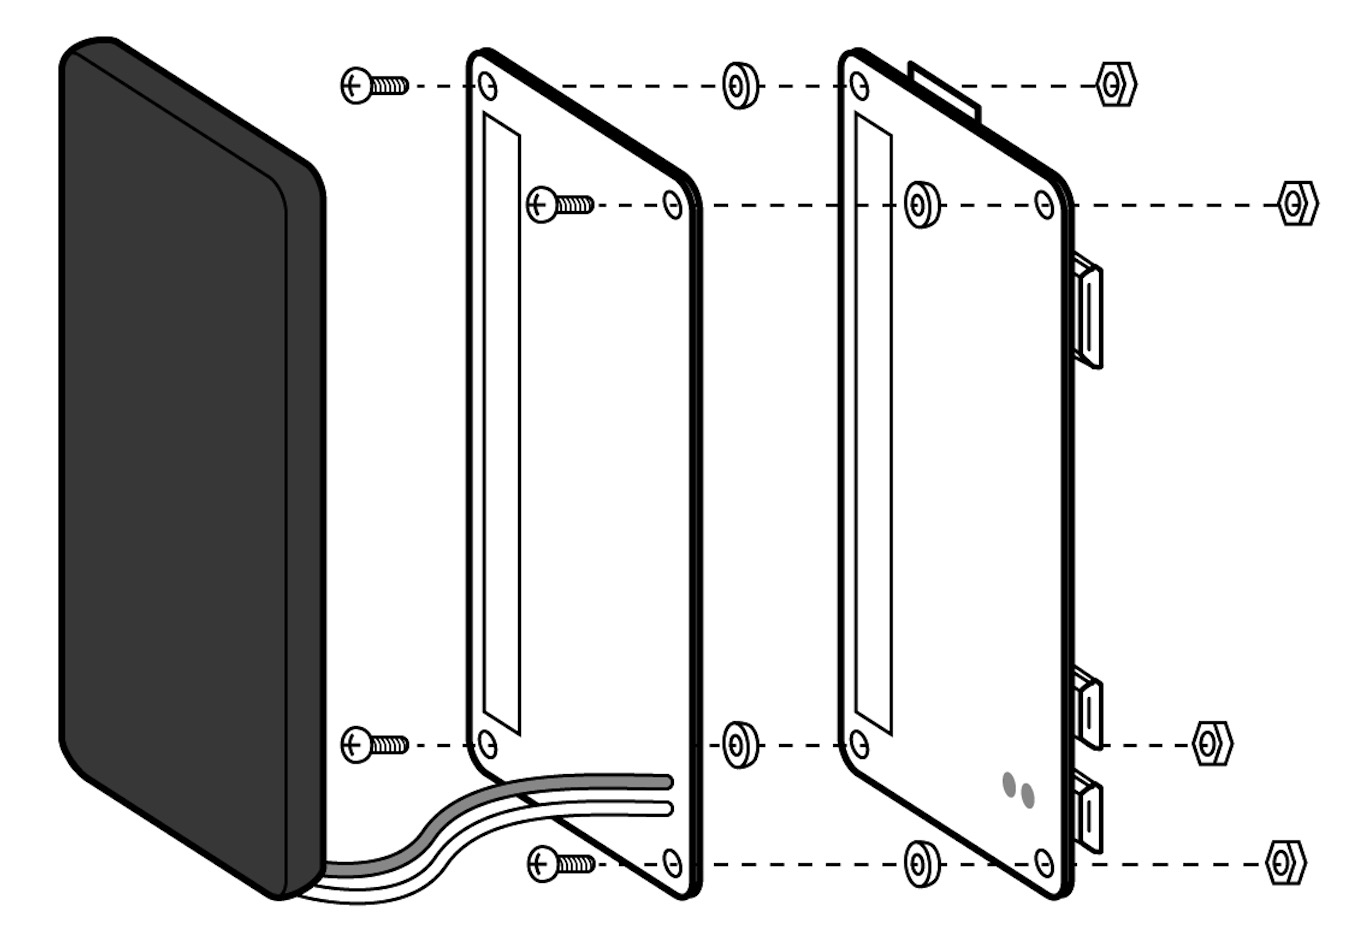
\includegraphics[width=0.4\textwidth]{ins.png} 
	\end{figure}
	通过查看树莓派板体的供电定义,发现可以从其四周的引脚引入供电,从而可以采用双层板设计,提高集成度,减少体积。目前市面上有成熟的方案(比如开源的
PiSugar项目),也可以自己制板但是需要添加电池稳压和监控电路。
			\begin{figure}[H] 
	\centering 
	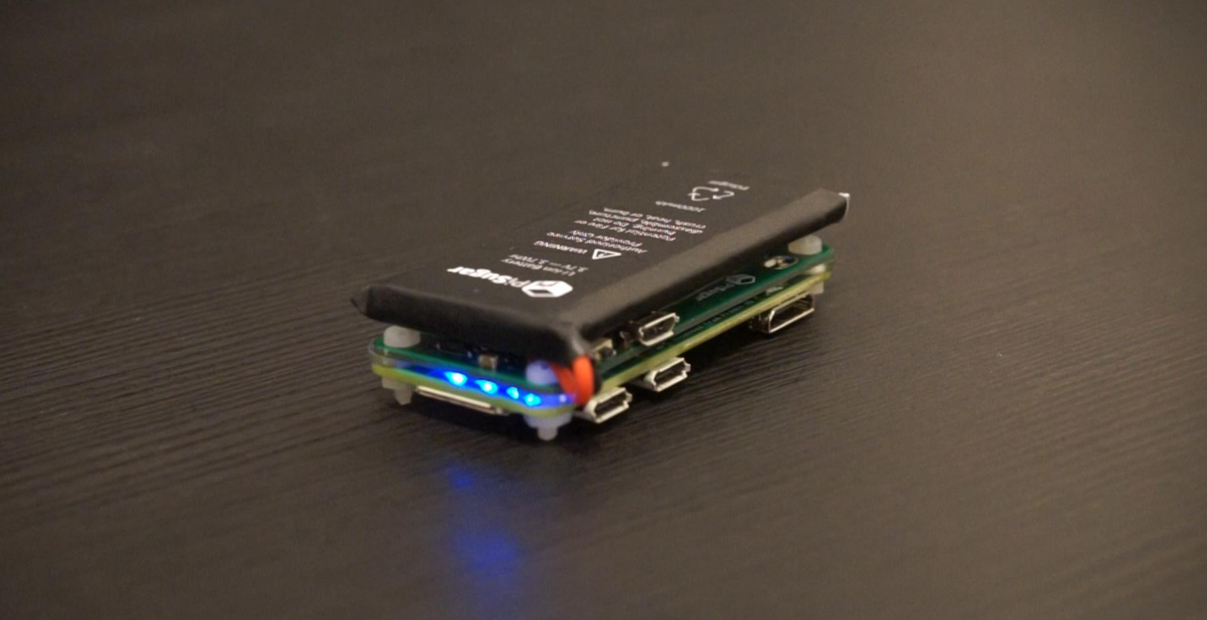
\includegraphics[width=0.4\textwidth]{demo2.png} 
	\end{figure}
 		
  \end{document}